\documentclass[11pt,twocolumn]{article}
\setlength{\topmargin}{0in}
\usepackage{graphicx} % Required for inserting images
\usepackage{titlesec}
\usepackage{multicol}

  
\title{\vspace{-4.0cm}Joint Optimization of Trajectory Planning and Task Scheduling in
Heterogeneous Multi-UAV System}
\author{\textbf{Pradeep Dalal}}
\date{\vspace{-5ex}}
\begin{document}
\maketitle
\vspace{50px}

{\LARGE \textbf{Abstract}}
\\\\
The use of unmanned aerial vehicles (UAV) as a new sensing paradigm is emerging for surveillance and tracking
applications, especially in the infrastructure-less environment. One such application of UAVs is in the construction industry where currently prevalent manual progress tracking results in schedule delays and cost overruns. Inthis paper, we develop a heterogeneous multi-UAV framework for progress tracking of large construction sites. The proposed framework consists of Edge UAV which coordinates the data relay of the visual sensor-equipped Inspection UAVs (I UAV s) to the cloud. Our framework jointlytakes into consideration the trajectory optimization of the Edge UAV and the stability of system queues. In particular, we develop a Distance and Access Latency Aware Trajectory (DLAT) optimization that generates a fair access schedule for I UAV s. In addition, a Lyapunov based online optimization ensures the system stability of the average queue backlogs for data offloading tasks. Through a message based mechanism, the coordination between the set of I UAV s and Edge UAV is ensured without any dependence on any central entity or message broadcasts.The performance of our proposed framework with joint optimization algorithm is validated by extensive simulation results in different parameter settings.\\\\
 \textbf{Keyword}: Path Planning, Task Scheduling, Data Of-floading, Construction Site Monitoring, Unmanned Aerial Vehicles (UAVs), Lyapunov Optimization

\section{Introduction}
The unmanned aerial vehicle (UAV) based solutions are emerging in various domains such as wireless sensing [1],
payload delivery [2], precision agriculture [3], help and rescue operations [4], etc. Moreover, with the current
trend of automation, sensing and information exchange in Industry 4.0, UAV based applications are also finding
their place in the construction industry especially for resource tracking and progress monitoring using aerial im-
agery. Such solutions are helpful in infrastructurelesslarge construction sites as they provide ease of deployment, quick access to the ground-truth data and higher reachability and coverage [5]. Further, the autonomous or semi-autonomous UAV based solutions could facilitate progress monitoring, building inspections (for cracks or other defects), safety inspections (to find any environ- mental hazards) and many more construction-specific audits automatically. The UAV based visual monitoring of 
under-construction projects also allows simultaneous observability of ground-truth data by different collaborating 
entities. Availability of such data and information helps in timely assessments that could reduce schedule delays,
cost overruns, resource wastage and financial losses which are not uncommon in construction projects.

A plausible solution to address the aforementioned challenges could be a Mobile Edge Computing (MEC) [6] based heterogeneous multi-UAV framework. Such a framework along with the prior geometric knowledge available about the construction site as gathered from a Building Information Model (BIM)[7] could help create an effective multi-UAV based visual monitoring system for con-
struction sites. As for any constrained environment, the optimization of computational resources is central to develop a solution. The integration of UAVs and MEC into a single framework could facilitate that with efficient data collection/processing from the UAV based dynamic sensors in infrastructure-less environments [8]. In addition,an MEC based framework can help to perform partial computation offloading wherein a part of data is processed by the UAVs while the rest gets offloaded to the cloud.

An MEC based UAV framework is not new and the deployment of the UAVs as base stations or edge servers is widely studied [9, 10]. These studies reflect on the flexibility in deployment of UAV based edge computing components. However, there is a problem of buffer overflow of UAVs due to the limited on-board processing and the shared bandwidth to transfer data to the cloud which leads to instability in the system. In addition, the dynamic nature of such systems with varying data traffic and continuous movement of UAVs makes it difficult to stabilize or control the system in a deterministic manner. Researchers have used online Lyapunov optimization[11] to address such system instabilities. Lyapunov optimization considers the stability of the system with timevarying data and optimizes time averages of system utility and queue backlogs.

In this paper, we address the challenges of deploying a heterogeneous multi-UAV system for construction site monitoring by the joint optimization of UAV trajectory planning and data offloading task scheduling. The proposed framework employs two types of UAVs viz. Inspection UAVs I UAV s and Mobile Edge UAVs (Edge UAV ).While the former is deployed as visual sensors to collect visual data from different locations of the site, the latter interacts and collects data from I UAV s, and offloads the same to the cloud. The core objective of the framework is to minimize the total energy consumption of the system while considering the data queue backlogs of I UAV sand Edge UAV and also jointly optimizing the trajectory
of the Edge UAV in accordance with the trajectories of I UAV s having minimum access latency and travel distance. The online resource management such as transmission power and processor frequency of the Edge UAV is evolved using Lyapunov optimization (as in [12]).The rest of the paper is organised as follows: Section 2 presents the proposed heterogeneous multi-UAV framework for construction site monitoring. The overall system objective is discussed in Sections 3. Sections 4 and 5 discuss the trajectory optimization and Lyapunov based system stability, respectively. The simulation setup has been
presented in Section 6. Section 7 discusses the results gathered from the experiments while Section 8 concludesthe paper.
    
\section{Heterogeneous Multi-UAV Framework}
Figure ?? depicts the overall multi-UAV framework with all its components. The system consists of two heterogeneous UAVs i.e. a set of Inspection UAVs I UAV ={I UAV1, I UAV2, I UAV3, ....., I UAVN } and a Mobile Edge UAV (Edge UAV ). I UAV s are smaller in size and are more agile. They collect visual data from a set of Point of Interests (PoIs) denoted as L = {l1, l2, l3....lk} across the construction site. As the construction sites are infrastructure-less environments, there are limited Access Points (AP) available for connectivity to the cloud. Further, the I UAV s possess limited connectivity range that makes it difficult for them to transfer data to cloud directly. In addition, the I UAV s move in the 3D Cartesian coordinate system. The Edge UAV , which is larger in size and possesses higher computational capabilities, coordinates with the I UAV s to relay the data (after partially
processing the same) to the cloud. Edge UAV always maintains a constant height and thus its trajectory lies in
an horizontal plane.

The communication between I UAV and Edge UAV (A2A channel) has limited range and bandwidth. We have assumed the achievable data transmission rate of the I $UAV_{i}$ in a given time slot as $d_{i}^{off}$(t). Further, The height of the Edge UAV is h which is dependent on coverage range r and line of sight (LoS) loss caused due to environmental effects [13]. The A2A channel power gain (ζ) from I UAV to Edge UAV can be given as: 

\begin{equation}
    T = g0*(dis0/dist)^{a}
\end{equation}

where g0 is the path loss constant, dis0 is the reference distance, dist distance between the UAVs, and a is the path loss exponent.

\subsection{Data collection and offloading}
Each PoI (li) is a tuple (< di, ψi >) where di specifies the amount of data (images) to be collected and ψi denotes the coordinates of the site locations in 3D space. The sequence
of PoIs to be visited is provided to I UAV s and same is also shared with the Edge UAV . During the traversal along the sequence of PoIs, the limited buffer may make the I UAV wait at some PoIs along the trajectory until it offloads the data to the Edge UAV .The Edge UAV can communicate with one of the I $UAV_{i}$ in a time slot. The data gathered by each of the I $UAV_{i}$ in a time slot t is denoted by $A_{i}$(t). $Q_{i}$(t) represents the queue of the I UAVi and $d_{i}^{off}$(t) denotes the amount of data offloaded to the Edge UAV by the I$UAV_{i}$
in time-slot t. The recursive equation to update
the $Q_{i}$(t) is as follows:.
\begin{equation} 
Q_{i}(t + 1) = max(Q_{i}(t) - d_{i}^{off}(t), 0) + A_{i}(t) 
\end{equation}
The Edge UAV accepts data from the selected I $UAV_{i}$ in the time-slot t in its queue L(t). The following equation updates L(t) recursively:
\begin{equation}
    L(t + 1) = max(L(t) - c(t) - d_{edge}^{off}(t), 0) + A_{edge}(t) 
\end{equation}
where Aedge(t) is the data arrived from the selected  I $UAV_{i}$ in time-slot t, c(t) is the data processed by the Edge UAV in time-slot t, and $d_{edge}^{off}$(t) is the number of bits offloaded to the cloud in time-slot t.

\section{System Objective}
In the proposed framework, the offloading of data happens at two stages - 1) from I UAVi to Edge UAV and 2) from Edge UAV to the cloud. Our main focus is to achieve the end-to-end data offloading to the cloud by minimizing the total energy consumption of the whole system (Esystem)
which is defined as:
\begin{equation}
    E_{system}(t) = E_{edge}^{transition}(t) + E_{edge}^{Comm}(t) +  E_{i}^{Comm}(t) 
\end{equation}

where $E_{edge}^{transition}(t)$ is the transition energy of the Edge UAV , $E_{edge}^{Comm}(t)$ is a communication energy of the Edge UAV and $E_{edge}^{Comm}(t)$ is the communication energy of the $i^{th}I$ $UAV_{i}$ Further, we discuss the various components of Esystem
along with the expressions to calculate the same.\cite{harnad2004access}
\\ \\\\
\subsection{Transition energy of Edge-UAV}
The transition energy of Edge UAV refers to the energy consumed in moving from one location to another. The transition energy of the Edge UAV is given as:

\begin{equation}
    E_{edge}^{transition} = k||vel(t)||^{2}
\end{equation}

where k is a constant that depends on the total mass of the Edge-UAV and vel(t) is the velocity of I-UAV.

\subsection{Communication energy of Edge-UAV}
Edge UAV offloads the data to cloud through a wireless channel [14]. The communication energy consumed to transmit the data to the cloud is given as:

\begin{equation}
    E_{edge}^{Comm}= (2^{d_{edge}^{off}(t)/W∗τ} - 1)*T
\end{equation}

\subsection{Communication Energy of I-UAV}
The energy consumed for offloading the ${d_{edge}^{off}(t)}$ data bits at time slot t from the selected I $UAV_{i}$ to the Edge-UAV using the A2A channel of bandwidth W Hz is given similarly to Equation 6 as:

\begin{equation}
    E_{edge}^{Comm}= (2^{d_{edge}^{off}(t)/W∗τ} - 1)*T
\end{equation}

As the PoIs are predefined and the I UAV s follow a predetermined path, the energy consumed or the movement of I UAV s are not taken into consideration.\cite{sharrif2011aloe}

Given the energy of the system, our goal is to find the optimal parameter values so as to minimize the expected cumulative energy across the time horizon. The system policy in every time-slot t can be given by X(t) ={ $F_{edge}$(t), $p_{i}$(t), $S_{edge}$(t), $P_{edge}$(t)}. 

\section{Algorithm}

Input: Trajectories of all I UAVi and list of PoIs li
Time, t = 0
while t ≤ T do
1. Estimate the {Qi(t)} N i=1and {Si(t)} N i=1
2. Select the i th I UAVi to offload data using P2
3. Compute and offload ${d_{edge}^{off}(t)}$for I UAVi using P 
\\3.1 to Edge UAV \\
4. Update Qi(t) \\
5. Transmit status message to Edge UAV\\
6. Compute and offload d of f edge(t) as using P 3.2 \\
7. Update L(t)\\
8. t=t+1

\\\\
\begin{figure}
\centering
\begin{subfigure}{.5\textwidth}
  \centering
  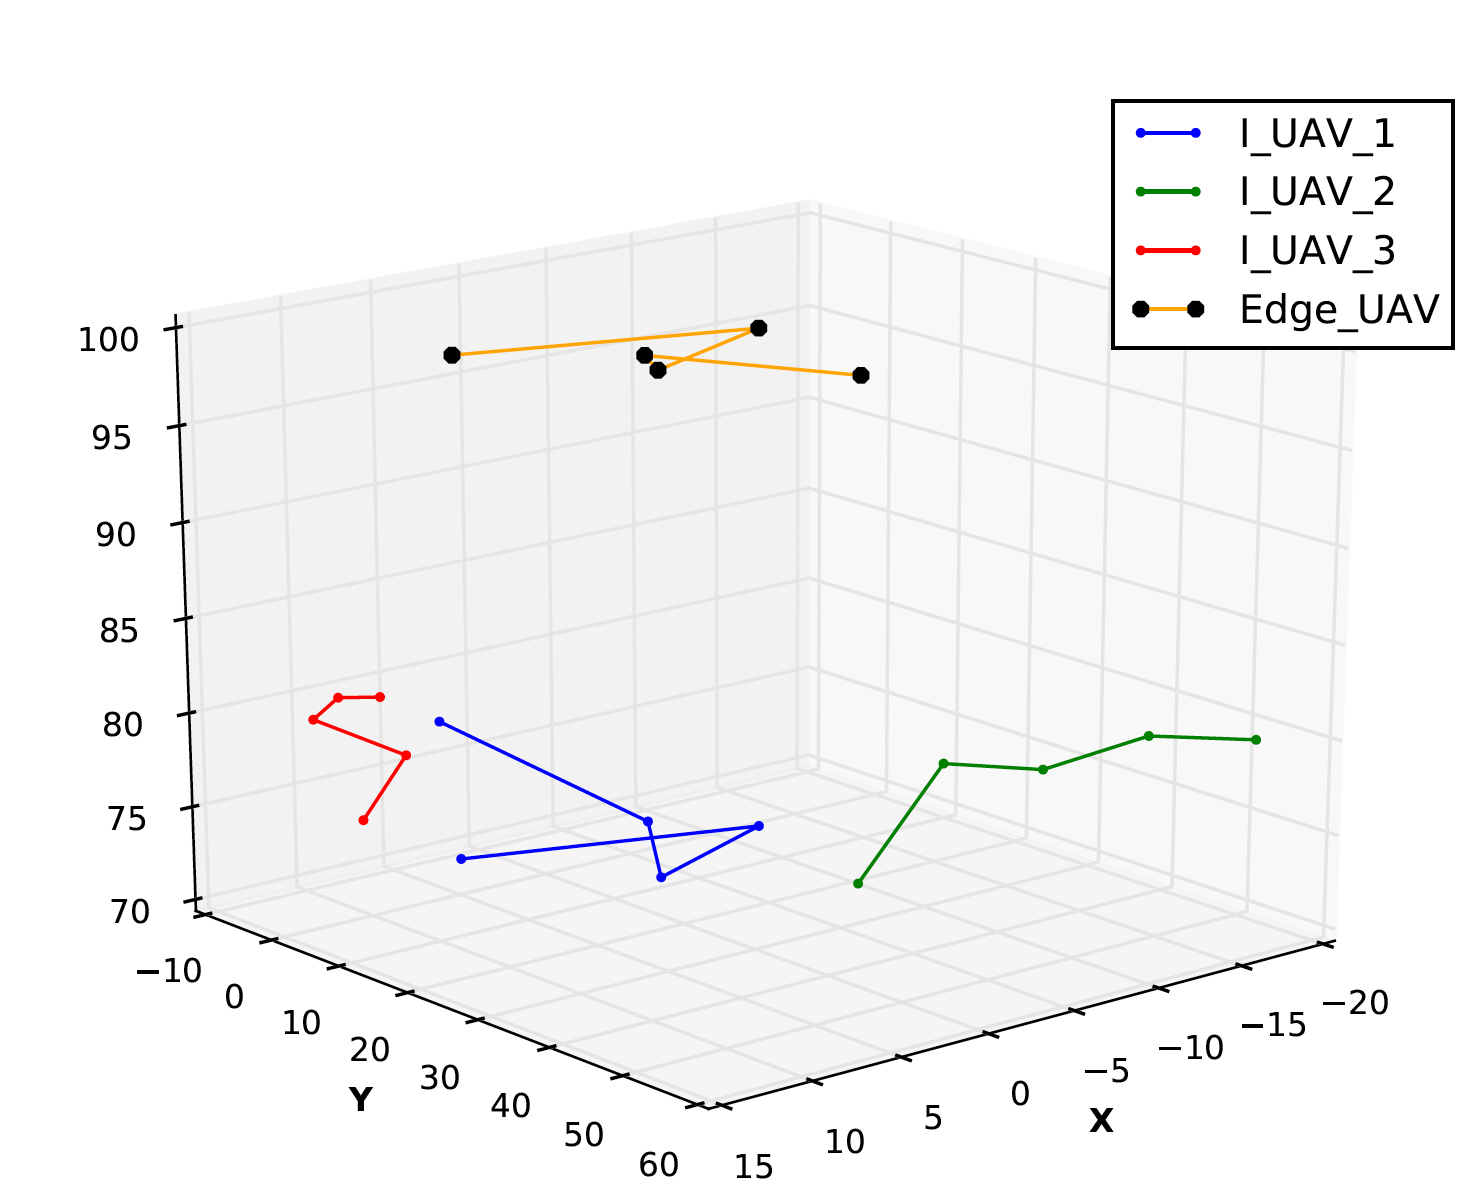
\includegraphics[width=.4\linewidth]{fig1.png}
  \label{fig:sub1}
\end{subfigure}%
\begin{subfigure}{.5\textwidth}
  \centering
  \includegraphics[width=.4\linewidth]{fig2.png}
  \label{fig:sub2}
\end{subfigure}
\label{fig:test}
\end{figure}

\section{Experimantation}
In this section, we present the simulation setup to validate the efficacy of our proposed Distance and Latency Aware Trajectory Optimization with Lyapunov based system utility. The pre-computed trajectories of each of the I UAVi are shared with the Edge UAV before the sim-
ulation starts. The simulation parameters are listed in Table 1.


\bibliographystyle{plain}
\bibliography{sample}

\end{document}
